\newpage
\subsection{Caso d'uso UC12: Menù profilo utente}
\label{UC12}

\begin{figure}[ht]
	\centering
	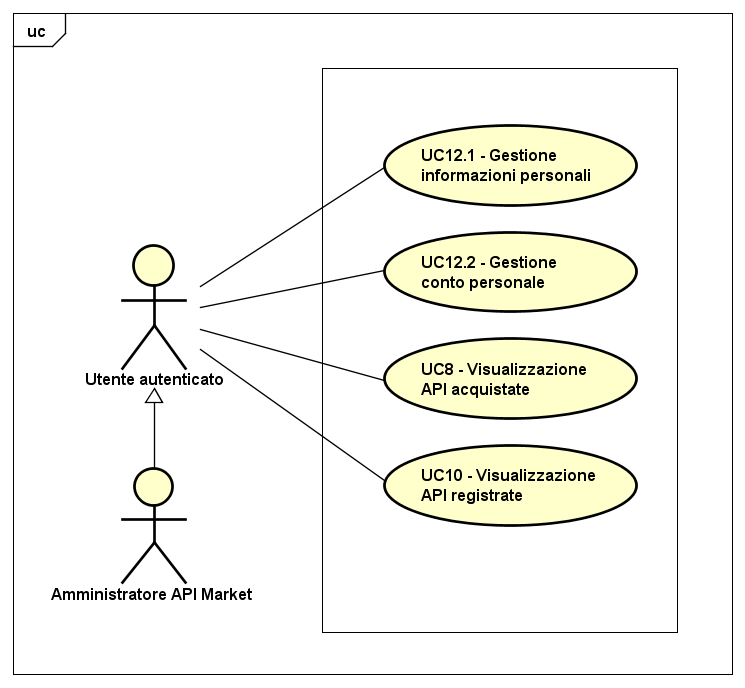
\includegraphics[scale=0.45]{UML/UC12.png}
	\caption{UC12 - Menù profilo utente}
\end{figure}
\FloatBarrier
\begin{longtable}{ l | p{11cm}}
	\hline
	\rowcolor{Gray}
	 \multicolumn{2}{c}{UC12 - Menù profilo utente} \\
	 \hline
	 \textbf{Attori} & Utente autenticato  \\
	\textbf{Descrizione} & L’attore può visualizzare e modificare i dati relativi all'account registrato \\
	\textbf{Pre-Condizioni} & L’attore è nel menù per la gestione del profilo \\
	\textbf{Post-Condizioni} & L’attore ha effettuato operazioni di gestione del proprio profilo \\
	\textbf{Scenario Principale} & 
	\begin{enumerate*}[label=(\arabic*.),itemjoin={\newline}]
		\item L'attore può gestire le proprie informazioni personali (UC12.1)
		\item L'attore può gestire il metodo di pagamento (UC12.2)
		\item L'attore può visualizzare le API acquistate (UC8)
		\item L'attore può interagire con le API da lui registrate e fornite sul marketplace (UC10)
	\end{enumerate*}\\
\end{longtable}

\subsubsection{Caso d'uso UC12.1: Gestione informazioni personali}
\label{UC12_1}

\begin{minipage}{\linewidth}
	\begin{tabular}{ l | p{11cm}}
		\hline
		\rowcolor{Gray}
		\multicolumn{2}{c}{UC12.1 - Gestione informazioni personali} \\
		\hline
		\textbf{Attori} & Utente autenticato \\
		\textbf{Descrizione} & L'attore può gestire le proprie informazioni personali\\
		\textbf{Pre-Condizioni} & L'attore si trova nel menù relativo alla gestione delle informazioni personali del profilo\\
		\textbf{Post-Condizioni} & L'attore ha effettuato operazioni di gestione di informazioni personali \\
		\textbf{Scenario Principale} & 
		\begin{enumerate*}[label=(\arabic*.),itemjoin={\newline}]
			\item L'attore può visualizzare le informazioni personali (UC12.1.1)
			\item L'attore può modificare le informazioni personali (UC12.1.2)
		\end{enumerate*}
	\end{tabular}
\end{minipage}

\newpage
\paragraph{Caso d'uso UC12.1.1: Visualizzazione info personali profilo utente}
\label{UC12_1_1}
\begin{figure}[ht]
	\centering
	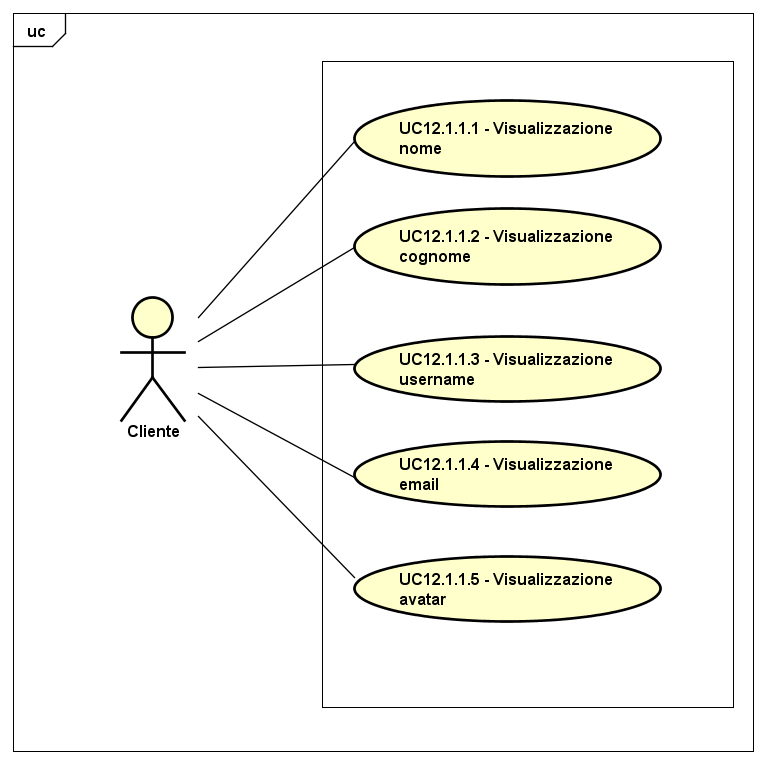
\includegraphics[scale=0.45]{UML/UC12_1_1.png}
	\caption{UC12.1.1: Visualizzazione info personali profilo utente}
\end{figure}
\FloatBarrier
\begin{tabular}{ l | p{11cm}}
	\hline
	\rowcolor{Gray}
	\multicolumn{2}{c}{UC12.1.1 - Visualizzazione info personali profilo utente} \\
	\hline
	\textbf{Attori} & Utente autenticato \\
	\textbf{Descrizione} & L'attore può visualizzare le informazioni personali relative al proprio account registrato\\
	\textbf{Pre-Condizioni} & L'attore è nella schermata di gestione informazioni personali\\
	\textbf{Post-Condizioni} & L'attore ha visualizzato le proprie informazioni personali \\
	\textbf{Scenario Principale} & 
	\begin{enumerate*}[label=(\arabic*.),itemjoin={\newline}]
		\item L'attore visualizza il nome (UC12.1.1.1)
		\item L'attore visualizza il cognome (UC12.1.1.2)
		\item L'attore visualizza lo username (UC12.1.1.3)
		\item L'attore visualizza l'email (UC12.1.1.4)
		\item L'attore visualizza l'immagine del profilo (UC12.1.1.5)
	\end{enumerate*}
\end{tabular}

\subparagraph{Caso d'uso UC12.1.1.1: Visualizzazione nome}
\label{UC12_1_1_1}

\begin{minipage}{\linewidth}
\begin{tabular}{ l | p{11cm}}
	\hline
	\rowcolor{Gray}
	\multicolumn{2}{c}{UC12.1.1.1 - Visualizzazione nome} \\
	\hline
	\textbf{Attori} & Utente autenticato \\
	\textbf{Descrizione} & L'attore può visualizzare il nome\\
	\textbf{Pre-Condizioni} & L'attore è nella schermata di visualizzazione informazioni personali\\
	\textbf{Post-Condizioni} & L'attore ha visualizzato il proprio nome \\
	\textbf{Scenario Principale} & 
	\begin{enumerate*}[label=(\arabic*.),itemjoin={\newline}]
		\item L'attore visualizza il proprio nome
	\end{enumerate*}
\end{tabular}
\end{minipage}

\subparagraph{Caso d'uso UC12.1.1.2: Visualizzazione cognome}
\label{UC12_1_1_2}

\begin{minipage}{\linewidth}
	\begin{tabular}{ l | p{11cm}}
		\hline
		\rowcolor{Gray}
		\multicolumn{2}{c}{UC12.1.1.2 - Visualizzazione cognome} \\
		\hline
		\textbf{Attori} & Utente autenticato \\
		\textbf{Descrizione} & L'attore può visualizzare il cognome\\
		\textbf{Pre-Condizioni} & L'attore è nella schermata di visualizzazione informazioni personali\\
		\textbf{Post-Condizioni} & L'attore ha visualizzato il proprio cognome \\
		\textbf{Scenario Principale} & 
		\begin{enumerate*}[label=(\arabic*.),itemjoin={\newline}]
			\item L'attore visualizza il proprio cognome
		\end{enumerate*}
	\end{tabular}
\end{minipage}

\subparagraph{Caso d'uso UC12.1.1.3: Visualizzazione username}
\label{UC12_1_1_3}
\begin{minipage}{\linewidth}
	\begin{tabular}{ l | p{11cm}}
		\hline
		\rowcolor{Gray}
		\multicolumn{2}{c}{UC12.1.1.3 - Visualizzazione username} \\
		\hline
		\textbf{Attori} & Utente autenticato \\
		\textbf{Descrizione} & L'attore può visualizzare lo username\\
		\textbf{Pre-Condizioni} & L'attore è nella schermata di visualizzazione informazioni personali\\
		\textbf{Post-Condizioni} & L'attore ha visualizzato il proprio username \\
		\textbf{Scenario Principale} & 
		\begin{enumerate*}[label=(\arabic*.),itemjoin={\newline}]
			\item L'attore visualizza il proprio username
		\end{enumerate*}
	\end{tabular}
\end{minipage}

\subparagraph{Caso d'uso UC12.1.1.4: Visualizzazione email}
\label{UC12_1_1_4}
\begin{minipage}{\linewidth}
	\begin{tabular}{ l | p{11cm}}
		\hline
		\rowcolor{Gray}
		\multicolumn{2}{c}{UC12.1.1.4 - Visualizzazione email} \\
		\hline
		\textbf{Attori} & Utente autenticato \\
		\textbf{Descrizione} & L'attore può visualizzare l'indirizzo email associato al proprio account\\
		\textbf{Pre-Condizioni} & L'attore è nella schermata di visualizzazione informazioni personali\\
		\textbf{Post-Condizioni} & L'attore ha visualizzato la propria email \\
		\textbf{Scenario Principale} & 
		\begin{enumerate*}[label=(\arabic*.),itemjoin={\newline}]
			\item L'attore visualizza la propria email
		\end{enumerate*}
	\end{tabular}
\end{minipage}

\subparagraph{Caso d'uso UC12.1.1.5: Visualizzazione immagine del profilo}
\label{UC12_1_1_5}
\begin{minipage}{\linewidth}
	\begin{tabular}{ l | p{11cm}}
		\hline
		\rowcolor{Gray}
		\multicolumn{2}{c}{UC12.1.1.5 - Visualizzazione immagine del profilo} \\
		\hline
		\textbf{Attori} & Utente autenticato \\
		\textbf{Descrizione} & L'attore può visualizzare l'immagine del profilo\\
		\textbf{Pre-Condizioni} & L'attore è nella schermata di visualizzazione informazioni personali\\
		\textbf{Post-Condizioni} & L'attore ha visualizzato l'immagine del proprio profilo \\
		\textbf{Scenario Principale} & 
		\begin{enumerate*}[label=(\arabic*.),itemjoin={\newline}]
			\item L'attore visualizza l'immagine del proprio profilo
		\end{enumerate*}
	\end{tabular}
\end{minipage}

\newpage
\paragraph{Caso d'uso UC12.1.2: Modifica info personali profilo utente}
\label{UC12_1_2}
\begin{figure}[ht]
	\centering
	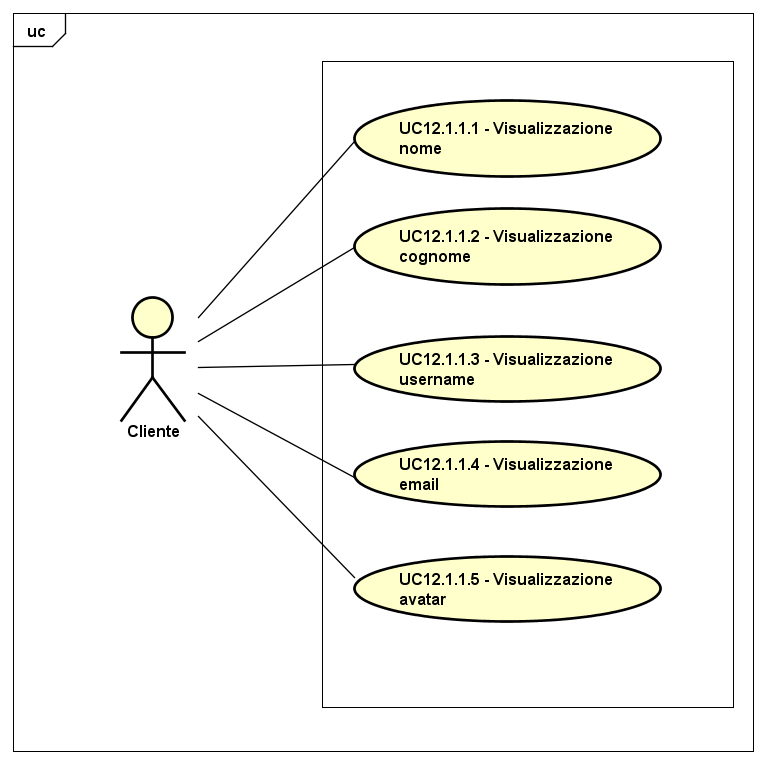
\includegraphics[scale=0.45]{UML/UC12_1_1.png}
	\caption{UC12.1.2: Modifica info personali profilo utente}
\end{figure}
\FloatBarrier
\begin{tabular}{ l | p{11cm}}
	\hline
	\rowcolor{Gray}
	\multicolumn{2}{c}{UC12.1.2 - Modifica info personali profilo utente} \\
	\hline
	\textbf{Attori} & Utente autenticato \\
	\textbf{Descrizione} & L'attore può modificare le informazioni personali relative al proprio profilo utente\\
	\textbf{Pre-Condizioni} & L'attore è nella schermata di gestione informazioni personali\\
	\textbf{Post-Condizioni} & L'attore ha modificato le proprie informazioni personali \\
	\textbf{Scenario Principale} & 
	\begin{enumerate*}[label=(\arabic*.),itemjoin={\newline}]
		\item L'attore può modificare il nome (UC12.1.2.1)
		\item L'attore può modificare il cognome (UC12.1.2.2)
		\item L'attore può modificare lo username (UC12.1.2.3)
		\item L'attore può modificare l'email (UC12.1.2.4)
		\item L'attore può modificare l'immagine del profilo (UC12.1.2.5)
		\item L'attore può confermare le modifiche effettuate (UC12.1.2.6)
	\end{enumerate*}\\
	\textbf{Scenari Alternativi} & 
	\begin{enumerate*}[label=(\arabic*.),itemjoin={\newline}]
		\item L'attore visualizza gli errori rilevati nelle modifiche richieste (UC12.1.2.7)
	\end{enumerate*}\\
\end{tabular}

\subparagraph{Caso d'uso UC12.1.2.1: Modifica nome}
\label{UC12_1_2_1}
\begin{minipage}{\linewidth}
	\begin{tabular}{ l | p{11cm}}
		\hline
		\rowcolor{Gray}
		\multicolumn{2}{c}{UC12.1.2.1 - Modifica nome} \\
		\hline
		\textbf{Attori} & Utente autenticato \\
		\textbf{Descrizione} & L'attore può modificare il nome\\
		\textbf{Pre-Condizioni} & L'attore è nella schermata di modifica informazioni personali\\
		\textbf{Post-Condizioni} & L'attore ha modificato il nome \\
		\textbf{Scenario Principale} & 
		\begin{enumerate*}[label=(\arabic*.),itemjoin={\newline}]
			\item L'attore può inserire il nuovo nome
		\end{enumerate*}\\
	\end{tabular}
\end{minipage}

\subparagraph{Caso d'uso UC12.1.2.2: Modifica cognome}
\label{UC12_1_2_2}
\begin{minipage}{\linewidth}
	\begin{tabular}{ l | p{11cm}}
		\hline
		\rowcolor{Gray}
		\multicolumn{2}{c}{UC12.1.2.2 - Modifica cognome} \\
		\hline
		\textbf{Attori} & Utente autenticato \\
		\textbf{Descrizione} & L'attore può modificare il cognome\\
		\textbf{Pre-Condizioni} & L'attore è nella schermata di modifica informazioni personali\\
		\textbf{Post-Condizioni} & L'attore ha modificato il cognome \\
		\textbf{Scenario Principale} & 
		\begin{enumerate*}[label=(\arabic*.),itemjoin={\newline}]
			\item L'attore può inserire il nuovo cognome
		\end{enumerate*}\\
	\end{tabular}
\end{minipage}

\subparagraph{Caso d'uso UC12.1.2.3: Modifica username}
\label{UC12_1_2_3}
\begin{minipage}{\linewidth}
	\begin{tabular}{ l | p{11cm}}
		\hline
		\rowcolor{Gray}
		\multicolumn{2}{c}{UC12.1.2.3 - Modifica username} \\
		\hline
		\textbf{Attori} & Utente autenticato \\
		\textbf{Descrizione} & L'attore può modificare lo username\\
		\textbf{Pre-Condizioni} & L'attore è nella schermata di modifica informazioni personali\\
		\textbf{Post-Condizioni} & L'attore ha modificato lo username\\
		\textbf{Scenario Principale} & 
		\begin{enumerate*}[label=(\arabic*.),itemjoin={\newline}]
			\item L'attore può inserire il nuovo username per il profilo
		\end{enumerate*}\\
	\end{tabular}
\end{minipage}

\subparagraph{Caso d'uso UC12.1.2.4: Modifica email}
\label{UC12_1_2_4}
\begin{minipage}{\linewidth}
	\begin{tabular}{ l | p{11cm}}
		\hline
		\rowcolor{Gray}
		\multicolumn{2}{c}{UC12.1.2.4 - Modifica email} \\
		\hline
		\textbf{Attori} & Utente autenticato \\
		\textbf{Descrizione} & L'attore può modificare l'email associata all'account registrato\\
		\textbf{Pre-Condizioni} & L'attore è nella schermata di modifica informazioni personali\\
		\textbf{Post-Condizioni} & L'attore ha modificato l'email \\
		\textbf{Scenario Principale} & 
		\begin{enumerate*}[label=(\arabic*.),itemjoin={\newline}]
			\item L'attore può inserire la nuova email da associare al proprio profilo
		\end{enumerate*}\\
	\end{tabular}
\end{minipage}

\subparagraph{Caso d'uso UC12.1.2.5: Modifica immagine profilo}
\label{UC12_1_2_5}
\begin{minipage}{\linewidth}
	\begin{tabular}{ l | p{11cm}}
		\hline
		\rowcolor{Gray}
		\multicolumn{2}{c}{UC12.1.2.5 - Modifica immagine profilo} \\
		\hline
		\textbf{Attori} & Utente autenticato \\
		\textbf{Descrizione} & L'attore può modificare l'immagine del proprio profilo\\
		\textbf{Pre-Condizioni} & L'attore è nella schermata di modifica informazioni personali\\
		\textbf{Post-Condizioni} & L'attore ha modificato l'immagine del proprio profilo \\
		\textbf{Scenario Principale} & 
		\begin{enumerate*}[label=(\arabic*.),itemjoin={\newline}]
			\item L'attore può inserire una nuova immagine del profilo
		\end{enumerate*}\\
	\end{tabular}
\end{minipage}

\subparagraph{Caso d'uso UC12.1.2.6: Conferma modifiche info profilo}
\label{UC12_1_2_6}
\begin{minipage}{\linewidth}
	\begin{tabular}{ l | p{11cm}}
		\hline
		\rowcolor{Gray}
		\multicolumn{2}{c}{UC12.1.2.6 - Conferma modifiche info profilo} \\
		\hline
		\textbf{Attori} & Utente autenticato \\
		\textbf{Descrizione} & L'attore può confermare le modifiche effettuate alle proprie informazioni personali\\
		\textbf{Pre-Condizioni} & L'attore è nella schermata di modifica informazioni personali\\
		\textbf{Post-Condizioni} & L'attore ha confermato le modifiche effettuate \\
		\textbf{Scenario Principale} & 
		\begin{enumerate*}[label=(\arabic*.),itemjoin={\newline}]
			\item L'attore può confermare le modifiche effettuate, visualizzando il messaggio di successo e venendo reindirizzato al menù relativo al profilo utente (UC12)
		\end{enumerate*}\\
	\end{tabular}
\end{minipage}

\subparagraph{Caso d'uso UC12.1.2.7: Errore modifiche info profilo}
\label{UC12_1_2_7}
\begin{minipage}{\linewidth}
	\begin{tabular}{ l | p{11cm}}
		\hline
		\rowcolor{Gray}
		\multicolumn{2}{c}{UC12.1.2.7 - Errore modifiche info profilo} \\
		\hline
		\textbf{Attori} & Utente autenticato \\
		\textbf{Descrizione} & L'attore visualizza un messaggio d'errore che indica il fallimento delle operazioni di modifica dati personali\\
		\textbf{Pre-Condizioni} & L'attore è nella schermata di modifica informazioni personali\\
		\textbf{Post-Condizioni} & L'attore ha confermato le modifiche effettuate, ma esse non sono valide\\
		\textbf{Scenario Principale} & 
		\begin{enumerate*}[label=(\arabic*.),itemjoin={\newline}]
			\item L'attore può visualizzare un messaggio d'errore che segnala i dati inseriti che non risultano validi
		\end{enumerate*}\\
	\end{tabular}
\end{minipage}

\subsubsection{Caso d'uso UC12.2: Gestione metodo di pagamento}
\label{UC12_2}

\begin{minipage}{\linewidth}
	\begin{tabular}{ l | p{11cm}}
		\hline
		\rowcolor{Gray}
		\multicolumn{2}{c}{UC12.2 - Gestione metodo di pagamento} \\
		\hline
		\textbf{Attori} & Utente autenticato \\
		\textbf{Descrizione} & L'attore può gestire il proprio credito \\
		\textbf{Pre-Condizioni} & L'attore si trova nel menù relativo alla gestione del metodo di pagamento\\
		\textbf{Post-Condizioni} & L'attore ha effettuato operazioni relative al metodo di pagamento \\
		\textbf{Scenario Principale} & 
		\begin{enumerate*}[label=(\arabic*.),itemjoin={\newline}]
			\item L'attore può visualizzare il credito attuale presente nel proprio account (UC12.2.1)
			\item L'attore può effettuare un versamento per accrescere il proprio credito (UC12.2.2)
		\end{enumerate*}
	\end{tabular}
\end{minipage}

\paragraph{Caso d'uso UC12.2.1: Visualizzazione saldo}
\label{UC12_2_1}
\begin{minipage}{\linewidth}
	\begin{tabular}{ l | p{11cm}}
		\hline
		\rowcolor{Gray}
		\multicolumn{2}{c}{UC12.2.1 - Visualizzazione saldo} \\
		\hline
		\textbf{Attori} & Utente autenticato \\
		\textbf{Descrizione} & L'attore può visualizzare il credito attuale relativo al proprio account \\
		\textbf{Pre-Condizioni} & L'attore si trova nella schermata di visualizzazione saldo\\
		\textbf{Post-Condizioni} & L'attore ha visualizzato il proprio credito attuale \\
		\textbf{Scenario Principale} & 
		\begin{enumerate*}[label=(\arabic*.),itemjoin={\newline}]
			\item L'attore può visualizzare il saldo corrente relativo al proprio account
		\end{enumerate*}\\
	\end{tabular}
\end{minipage}

\paragraph{Caso d'uso UC12.2.2: Versamento saldo}
\label{UC12_2_2}
\begin{minipage}{\linewidth}
	\begin{tabular}{ l | p{11cm}}
		\hline
		\rowcolor{Gray}
		\multicolumn{2}{c}{UC12.2.2 - Versamento saldo} \\
		\hline
		\textbf{Attori} & Utente autenticato \\
		\textbf{Descrizione} & L'attore può incrementare il proprio credito per effettuare acquisti di API sulla piattaforma \\
		\textbf{Pre-Condizioni} & L'attore si trova nella schermata per effettuare il versamento\\
		\textbf{Post-Condizioni} & L'attore ha effettuato un versamento sul proprio saldo \\
		\textbf{Scenario Principale} & 
		\begin{enumerate*}[label=(\arabic*.),itemjoin={\newline}]
			\item L'attore può selezionare la cifra da accreditare sul proprio saldo (UC12.2.2.1)
			\item L'attore può confermare la somma selezionata e procedere con l'operazione di ricarica del credito personale (UC12.2.2.2)
		\end{enumerate*}\\
		\textbf{Scenari Alternativi} & \begin{enumerate*}[label=(\arabic*.),itemjoin={\newline}]
			\item L'attore può visualizzare un messaggio d'errore che segnala il fallimento dell'operazione di versamento sul saldo personale (UC12.2.2.3)
		\end{enumerate*}\\
	\end{tabular}
\end{minipage}

\subparagraph{Caso d'uso UC12.2.2.1: Selezione somma di accredito}
\label{UC12_2_2_1}
\begin{minipage}{\linewidth}
	\begin{tabular}{ l | p{11cm}}
		\hline
		\rowcolor{Gray}
		\multicolumn{2}{c}{UC12.2.2.1 - Selezione somma di accredito} \\
		\hline
		\textbf{Attori} & Utente autenticato \\
		\textbf{Descrizione} & L'attore può selezionare la quantità di denaro da aggiungere al saldo attuale presente sul proprio account \\
		\textbf{Pre-Condizioni} & L'attore si trova nella schermata per effettuare il versamento\\
		\textbf{Post-Condizioni} & L'attore ha selezionato la somma da accreditare al proprio saldo \\
		\textbf{Scenario Principale} & 
		\begin{enumerate*}[label=(\arabic*.),itemjoin={\newline}]
			\item L'attore può selezionare la cifra da accreditare sul proprio saldo
		\end{enumerate*}\\
	\end{tabular}
\end{minipage}

\subparagraph{Caso d'uso UC12.2.2.2: Conferma accredito somma selezionata}
\label{UC12_2_2_2}
\begin{minipage}{\linewidth}
	\begin{tabular}{ l | p{11cm}}
		\hline
		\rowcolor{Gray}
		\multicolumn{2}{c}{UC12.2.2.2 - Conferma accredito somma selezionata} \\
		\hline
		\textbf{Attori} & Utente autenticato \\
		\textbf{Descrizione} & L'attore può confermare la somma indicata come accredito sul saldo personale del proprio account \\
		\textbf{Pre-Condizioni} & L'attore si trova nella schermata per effettuare il versamento\\
		\textbf{Post-Condizioni} & L'attore ha effettuato un versamento sul proprio saldo \\
		\textbf{Scenario Principale} & 
		\begin{enumerate*}[label=(\arabic*.),itemjoin={\newline}]
			\item L'attore può selezionare la cifra da accreditare sul proprio saldo
		\end{enumerate*}\\
	\end{tabular}
\end{minipage}

\subparagraph{Caso d'uso UC12.2.2.3: Fallimento ricarica saldo}
\label{UC12_2_2_3}
\begin{minipage}{\linewidth}
	\begin{tabular}{ l | p{11cm}}
		\hline
		\rowcolor{Gray}
		\multicolumn{2}{c}{UC12.2.2.3 - Fallimento ricarica saldo} \\
		\hline
		\textbf{Attori} & Utente autenticato \\
		\textbf{Descrizione} & L'attore fallisce il versamento sul saldo \\
		\textbf{Pre-Condizioni} & L'attore si trova nella schermata per effettuare il versamento\\
		\textbf{Post-Condizioni} & L'attore ha visualizzato un messaggio d'errore che segnala il fallimento relativo al versamento sul saldo personale \\
		\textbf{Scenario Principale} & 
		\begin{enumerate*}[label=(\arabic*.),itemjoin={\newline}]
			\item L'attore può visualizzare un messaggio d'errore indicante il fallimento della procedura di ricarica saldo 
		\end{enumerate*}\\
	\end{tabular}
\end{minipage}